%%%%%%%%%%%%%%%%%%%%%%%%%%%%%%%%%%%%%%%%%
% University/School Laboratory Report
% LaTeX Template
% Version 3.0 (4/2/13)
%
% This template has been downloaded from:
% http://www.LaTeXTemplates.com
%
% Original author:
% Linux and Unix Users Group at Virginia Tech Wiki 
% (https://vtluug.org/wiki/Example_LaTeX_chem_lab_report)
%
% License:
% CC BY-NC-SA 3.0 (http://creativecommons.org/licenses/by-nc-sa/3.0/)
%
%%%%%%%%%%%%%%%%%%%%%%%%%%%%%%%%%%%%%%%%%

%----------------------------------------------------------------------------------------
%	PACKAGES AND DOCUMENT CONFIGURATIONS
%----------------------------------------------------------------------------------------

\documentclass{article}

\usepackage[version=3]{mhchem} % Package for chemical equation typesetting
\usepackage{siunitx} % Provides the \SI{}{} command for typesetting SI units

\usepackage{graphicx}
\usepackage{caption}
\usepackage{subcaption}

\usepackage{float}

\usepackage[T1]{fontenc} % allow small bold caps

\usepackage{listings}
\usepackage{color}

\definecolor{dkgreen}{rgb}{0,0.6,0}
\definecolor{gray}{rgb}{0.5,0.5,0.5}
\definecolor{mauve}{rgb}{0.58,0,0.82}

\lstset{frame=tb,
  language=Python,
  aboveskip=2mm,
  belowskip=2mm,
  showstringspaces=false,
  columns=flexible,
  basicstyle={\small\ttfamily},
  numbers=none,
  numberstyle=\tiny\color{gray},
  keywordstyle=\color{blue},
  commentstyle=\color{dkgreen},
  stringstyle=\color{mauve},
  breaklines=true,
  breakatwhitespace=true
  tabsize=2
}

\setlength\parindent{0pt} % Removes all indentation from paragraphs

\renewcommand{\labelenumi}{\alph{enumi}.} % Make numbering in the enumerate environment by letter rather than number (e.g. section 6)

\usepackage[margin=1in]{geometry}

\usepackage{amssymb}

%\usepackage{times} % Uncomment to use the Times New Roman font

%----------------------------------------------------------------------------------------
%	Title
%----------------------------------------------------------------------------------------

\begin{document}
\pagenumbering{gobble}

\title{6.036: Machine Learning}
\author{
  Ryan Lacey <rlacey@mit.edu>\\
}
        
\maketitle
        

\begin{enumerate}
\item[1.] 
	\begin{enumerate}
	\item[(a)]
		For each next $x$ there is no component of $\theta$ in the direction of $x$, so the dot product is zero. Perceptron classifies this as a mistake. This will occur $d$ times, each time fixing updating $\theta$ to correct the new mistake, which will not have to be fixed again. The feature vector ordering does matter because the dot product of any previously unseen $x$ with $\theta$ is zero until $\theta$ converges to a vector of ones.
\bigskip
	\item[(b)]
		$\theta$ converges to a vector of ones, ie. $\left[1_0, 1_1, 1_2, ..., 1_d\right]$
\bigskip
	\item[(c)]
		Bound on number of mistakes is $\dfrac{R^2}{\gamma^2}$\\
		
		$R \ge ||x^{(i)}||$\\
		$||x^{(i)}|| = 1$\\
		
		$\gamma = ||\theta||^{-1}$\\
		$\gamma = \sqrt{d}^{-1}$\\
		
		$\dfrac{R^2}{\gamma^2} = \dfrac{1}{\sqrt{d}^{-2}} = d$\\
		
		We respect our mistakes bound established in class and hit the maximum number of possible mistakes in this arrangement.
\bigskip
	\item[(d)]
		No, the number of mistakes will not depend upon the feature vector ordering. The passive aggressive function will update and thereafter correctly classify one point at a time, thereby requiring $d$ mistakes before all points are correctly classified. In the end we will converge to the same $\theta$ as perceptron. The hinge loss will be one until this convergence, for any ordering of the feature vectors, so passive aggressive will run analogous to the perceptron algorithm.
		
	\end{enumerate}
\newpage

\item[2.] 
	\begin{enumerate}
	\item[(a)] $\:$ \\
		\begin{figure}[!htb]
		\minipage{0.49\textwidth}
		  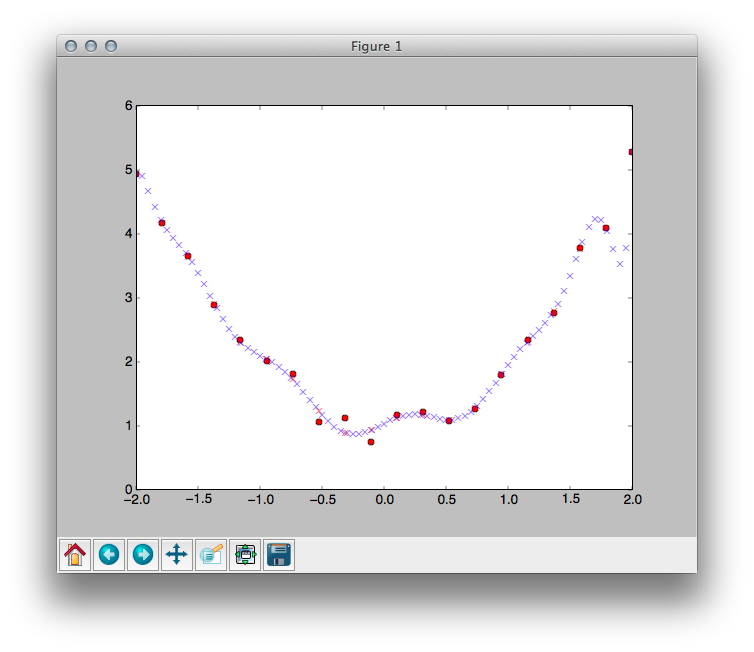
\includegraphics[width=\linewidth]{../images/Overfitting.png}
		  \caption{Line overfitting to training data points when regression parameters set to \\ \texttt{noisy\_quad\_fit(13, 0.00001)}}
		\endminipage\hfill
		\minipage{0.49\textwidth}
		  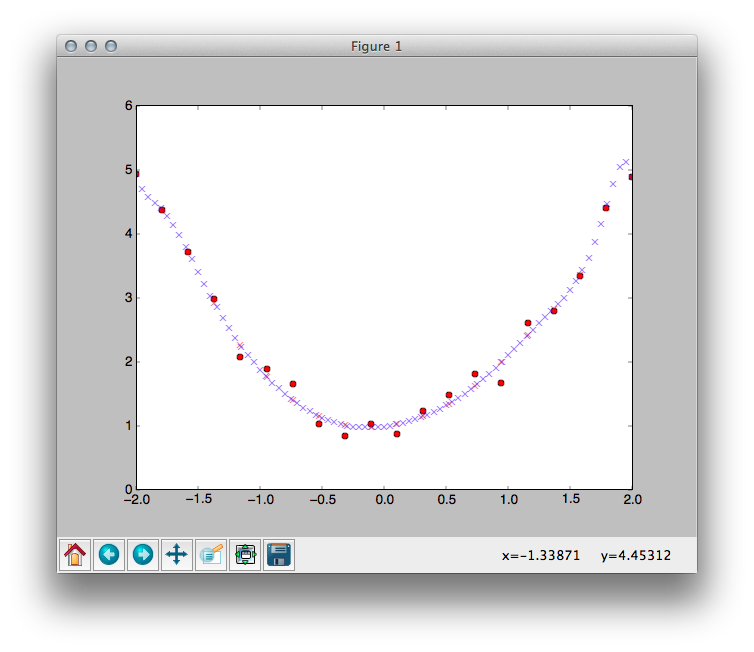
\includegraphics[width=\linewidth]{../images/Generalizable.png}
		  \caption{Line that generalizes well to test data when regression parameters set to \\ \texttt{noisy\_quad\_fit(13, 0.1)}}
		\endminipage\hfill
		\end{figure}

\newpage

	\item[(b)] $\:$ \\
		\begin{figure}[!htb]
		\minipage{0.49\textwidth}
		  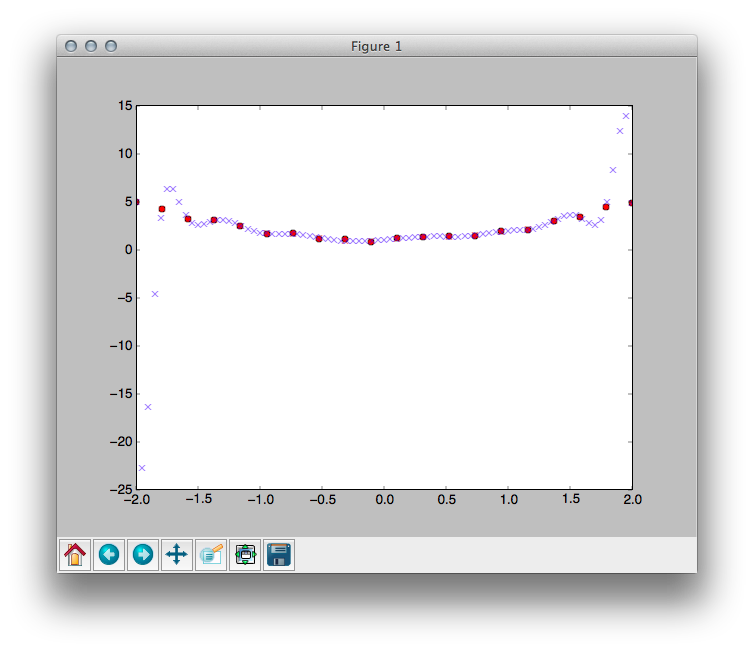
\includegraphics[width=\linewidth]{../images/Training.png}
		  \caption{Minimum training error = 0.0827554694891 at \texttt{order=18} and \texttt{regularization = 1e-06}}
		\endminipage\hfill
		\minipage{0.49\textwidth}
		  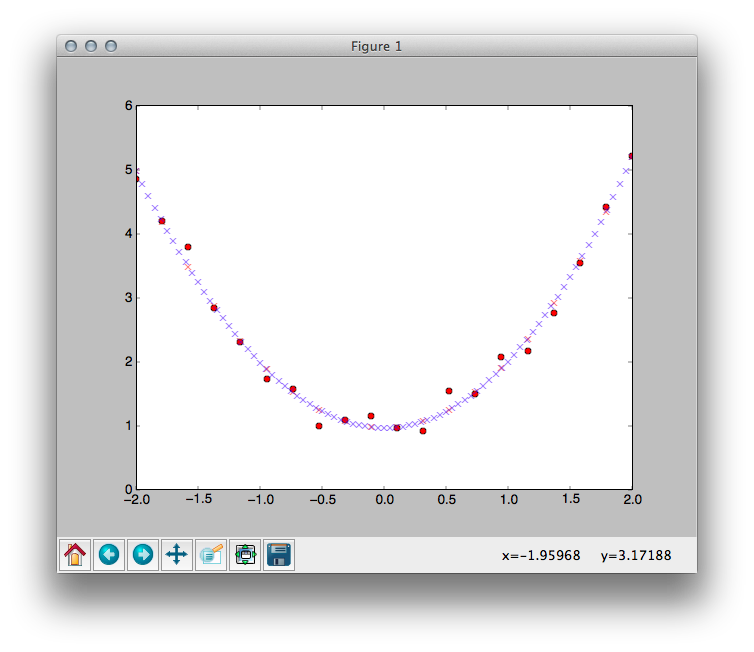
\includegraphics[width=\linewidth]{../images/Testing.png}
		  \caption{Minimum testing error = 0.0397647479675 at \texttt{order=3} and \texttt{regularization = 1e-06}}
		\endminipage\hfill
		\end{figure}
	\end{enumerate}

\bigskip

	\item[(c)]Sinusoid with noise\\
	
		Minimum training error = 0.0702075371943 at \texttt{order=17} and \texttt{regularization = 5e-06}\\
		Minimum testing error =  0.141655026216 at \texttt{order=10} and \texttt{regularization = 0.01}

\bigskip

	\item[(d)] No noise regressions\\
	
		Polynomial\\
			Minimum training error = 7.00892770489e-08 at \texttt{order=2} and \texttt{regularization = 1e-06}\\
			Minimum testing error =  7.02414684195e-08 at \texttt{order=2} and \texttt{regularization = 1e-06}\\
			
	Sinusoid\\
		Minimum training error = 0.0000484999916992 at \texttt{order=13} and \texttt{regularization = 1e-06}\\
		Minimum testing error =  0.000132456013403 at \texttt{order=13} and \texttt{regularization = 1e-06}\\
		
		Without noise the training and test data sets had the same optimal order and regularization parameter. This make sense because the points for both data sets were created in the same manner (an even distribution over some predefined space). The small, arguably negligible, differences in the error between the test and the training sets arises from the fact that they contained different quantities of points. Note the order of the polynomial is 2, which should be expected because the \texttt{vander} operation that determined the point locations results in a parabolic curve. It is also worth noting that although the error for the sinusoid is small, it is several magnitudes greater than that of the polynomial. This is because we use a polynomial to emulate the curvature of a sinusoid, which quickly plateaus in its ability to trace without being of a very high order.
\end{enumerate}

\end{document}